\documentclass[tikz, varwidth=600pt]{standalone}
\usepackage{amssymb, amsmath,bbm}

\standaloneenv{aaaa}

\begin{document}
	\begin{aaaa}
		\begin{center}	
		
		\fbox{%
			\begin{minipage}{0.85\linewidth}
				\centering
				\tikzset{every picture/.style={line width=0.75pt}} %set default line width to 0.75pt        
				\vspace{6pt} 
		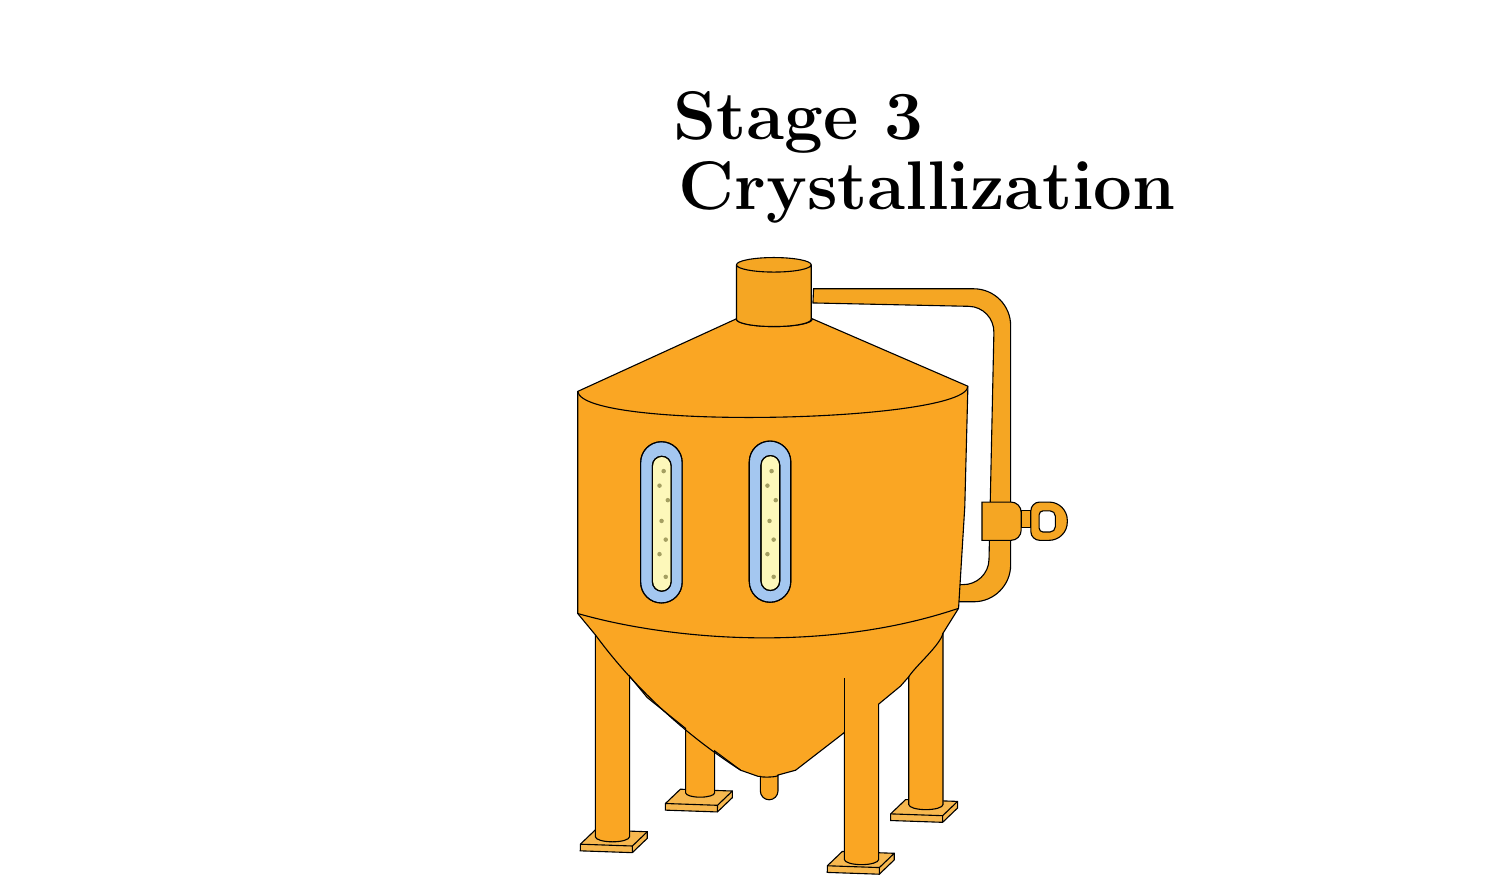
\begin{tikzpicture}[x=0.75pt,y=0.75pt,yscale=-1,xscale=1]
			
			% === Fixer un grand carré pour la taille de la page (même style que Step 1–2) ===
			\path[use as bounding box] (0,0) rectangle (700,400); % carré invisible mais fixe la taille
			%Shape: Path Data [id:dp740170980224085] 
			\draw  [fill={rgb, 255:red, 245; green, 166; blue, 35 }  ,fill opacity=1 ] (455.8,125.8) .. controls (465.63,125.8) and (473.6,133.77) .. (473.6,143.6) -- (473.6,258.8) .. controls (473.6,268.63) and (465.63,276.6) .. (455.8,276.6) -- (448.48,276.6) -- (448.41,268.28) -- (450.54,268.33) .. controls (457.37,268.47) and (463.03,263.05) .. (463.17,256.22) -- (465.52,146.88) .. controls (465.67,140.05) and (460.25,134.39) .. (453.42,134.25) -- (378.34,132.63) -- (378.64,125.8) -- (455.8,125.8) -- cycle ;
			%Shape: Cube [id:dp5541728812371717] 
			\draw  [fill={rgb, 255:red, 245; green, 166; blue, 35 }  ,fill opacity=0.8 ] (415.78,378.79) -- (422.97,371.91) -- (448.03,372.78) -- (448,375.98) -- (440.81,382.86) -- (415.75,381.99) -- cycle ; \draw   (448.03,372.78) -- (440.84,379.66) -- (415.78,378.79) ; \draw   (440.84,379.66) -- (440.81,382.86) ;
			%Shape: Cube [id:dp17416947613627154] 
			\draw  [fill={rgb, 255:red, 245; green, 166; blue, 35 }  ,fill opacity=0.8 ] (385.28,403.79) -- (392.47,396.91) -- (417.53,397.78) -- (417.5,400.98) -- (410.31,407.86) -- (385.25,406.99) -- cycle ; \draw   (417.53,397.78) -- (410.34,404.66) -- (385.28,403.79) ; \draw   (410.34,404.66) -- (410.31,407.86) ;
			%Shape: Cube [id:dp7638862186279323] 
			\draw  [fill={rgb, 255:red, 245; green, 166; blue, 35 }  ,fill opacity=0.8 ] (307.28,373.79) -- (314.47,366.91) -- (339.53,367.78) -- (339.5,370.98) -- (332.31,377.86) -- (307.25,376.99) -- cycle ; \draw   (339.53,367.78) -- (332.34,374.66) -- (307.28,373.79) ; \draw   (332.34,374.66) -- (332.31,377.86) ;
			%Shape: Cube [id:dp4600455976097241] 
			\draw  [fill={rgb, 255:red, 245; green, 166; blue, 35 }  ,fill opacity=0.8 ] (266.28,393.4) -- (273.47,386.52) -- (298.53,387.39) -- (298.5,390.59) -- (291.31,397.47) -- (266.25,396.6) -- cycle ; \draw   (298.53,387.39) -- (291.34,394.27) -- (266.28,393.4) ; \draw   (291.34,394.27) -- (291.31,397.47) ;
			%Shape: Path Data [id:dp4984379776478407] 
			\draw  [fill={rgb, 255:red, 250; green, 166; blue, 35 }  ,fill opacity=1 ] (453,172.75) -- (451.5,230.75) -- (448.5,279.75) -- (441,291.75) -- (441,374.28) .. controls (441,375.64) and (437.31,376.75) .. (432.75,376.75) .. controls (428.19,376.75) and (424.5,375.64) .. (424.5,374.28) -- (424.5,312.73) -- (420.5,317.25) -- (410,325.91) -- (410,400.78) .. controls (410,402.14) and (406.31,403.25) .. (401.75,403.25) .. controls (397.19,403.25) and (393.5,402.14) .. (393.5,400.78) -- (393.5,339.51) -- (392,340.75) -- (370,357.75) -- (361.5,360.07) -- (361.5,367.75) .. controls (361.5,370.1) and (359.6,372) .. (357.25,372) .. controls (354.9,372) and (353,370.1) .. (353,367.75) -- (353,360.75) -- (352,360.75) -- (343.5,357.75) -- (331,348.46) -- (331,368.65) .. controls (331,369.81) and (327.87,370.75) .. (324,370.75) .. controls (320.13,370.75) and (317,369.81) .. (317,368.65) -- (317,337.62) -- (298.5,322.75) -- (290,312.47) -- (290,389.78) .. controls (290,391.14) and (286.31,392.25) .. (281.75,392.25) .. controls (277.19,392.25) and (273.5,391.14) .. (273.5,389.78) -- (273.5,292.53) -- (265,282.25) -- (265,175.25) -- (341.5,140.25) -- (341.5,140.5) .. controls (341.5,142.43) and (349.67,144) .. (359.75,144) .. controls (369.83,144) and (378,142.43) .. (378,140.5) -- (378,140.25) -- (453,172.75) -- cycle (347.67,209.17) -- (347.67,266.83) .. controls (347.67,272.36) and (352.14,276.83) .. (357.67,276.83) .. controls (363.19,276.83) and (367.67,272.36) .. (367.67,266.83) -- (367.67,209.17) .. controls (367.67,203.64) and (363.19,199.17) .. (357.67,199.17) .. controls (352.14,199.17) and (347.67,203.64) .. (347.67,209.17) -- cycle (295.33,209.5) -- (295.33,267.17) .. controls (295.33,272.69) and (299.81,277.17) .. (305.33,277.17) .. controls (310.86,277.17) and (315.33,272.69) .. (315.33,267.17) -- (315.33,209.5) .. controls (315.33,203.98) and (310.86,199.5) .. (305.33,199.5) .. controls (299.81,199.5) and (295.33,203.98) .. (295.33,209.5) -- cycle ;
			%Shape: Can [id:dp22007502420139957] 
			\draw  [fill={rgb, 255:red, 245; green, 166; blue, 35 }  ,fill opacity=1 ] (377.5,114.25) -- (377.5,140.5) .. controls (377.5,142.43) and (369.44,144) .. (359.5,144) .. controls (349.56,144) and (341.5,142.43) .. (341.5,140.5) -- (341.5,114.25) .. controls (341.5,112.32) and (349.56,110.75) .. (359.5,110.75) .. controls (369.44,110.75) and (377.5,112.32) .. (377.5,114.25) .. controls (377.5,116.18) and (369.44,117.75) .. (359.5,117.75) .. controls (349.56,117.75) and (341.5,116.18) .. (341.5,114.25) ;
			%Curve Lines [id:da4915514043760123] 
			\draw    (265,282.25) .. controls (308.5,294.75) and (383.5,301.75) .. (448.5,279.75) ;
			%Curve Lines [id:da918344478950904] 
			\draw    (265,175.25) .. controls (267.5,194.25) and (452.5,190.25) .. (453,172.75) ;
			%Curve Lines [id:da7015792738779195] 
			\draw    (273.5,292.53) .. controls (277.5,297.75) and (300,329.75) .. (343.5,357.75) ;
			%Straight Lines [id:da26177027737321357] 
			\draw    (393.5,339.51) -- (393.5,313.25) ;
			%Curve Lines [id:da2507204405100264] 
			\draw    (424.5,312.73) .. controls (428,307.25) and (439.5,297.75) .. (441,291.75) ;
			%Curve Lines [id:da9174681435393754] 
			\draw    (353,360.75) .. controls (353,361.25) and (362,361.25) .. (361.5,360.07) ;
			%Shape: Circle [id:dp242588595185817] 
			\draw  [draw opacity=0][fill={rgb, 255:red, 0; green, 0; blue, 0 }  ,fill opacity=0.5 ] (306.33,264.58) .. controls (306.33,263.99) and (306.82,263.5) .. (307.42,263.5) .. controls (308.01,263.5) and (308.5,263.99) .. (308.5,264.58) .. controls (308.5,265.18) and (308.01,265.67) .. (307.42,265.67) .. controls (306.82,265.67) and (306.33,265.18) .. (306.33,264.58) -- cycle ;
			%Shape: Circle [id:dp053869881637099826] 
			\draw  [draw opacity=0][fill={rgb, 255:red, 0; green, 0; blue, 0 }  ,fill opacity=0.5 ] (303.33,253.65) .. controls (303.33,253.05) and (303.82,252.57) .. (304.42,252.57) .. controls (305.01,252.57) and (305.5,253.05) .. (305.5,253.65) .. controls (305.5,254.25) and (305.01,254.73) .. (304.42,254.73) .. controls (303.82,254.73) and (303.33,254.25) .. (303.33,253.65) -- cycle ;
			%Shape: Circle [id:dp23321530676438273] 
			\draw  [draw opacity=0][fill={rgb, 255:red, 0; green, 0; blue, 0 }  ,fill opacity=0.5 ] (306.33,246.65) .. controls (306.33,246.05) and (306.82,245.57) .. (307.42,245.57) .. controls (308.01,245.57) and (308.5,246.05) .. (308.5,246.65) .. controls (308.5,247.25) and (308.01,247.73) .. (307.42,247.73) .. controls (306.82,247.73) and (306.33,247.25) .. (306.33,246.65) -- cycle ;
			%Shape: Circle [id:dp5098212117846179] 
			\draw  [draw opacity=0][fill={rgb, 255:red, 0; green, 0; blue, 0 }  ,fill opacity=0.5 ] (304.33,237.65) .. controls (304.33,237.05) and (304.82,236.57) .. (305.42,236.57) .. controls (306.01,236.57) and (306.5,237.05) .. (306.5,237.65) .. controls (306.5,238.25) and (306.01,238.73) .. (305.42,238.73) .. controls (304.82,238.73) and (304.33,238.25) .. (304.33,237.65) -- cycle ;
			%Shape: Circle [id:dp36591736603179903] 
			\draw  [draw opacity=0][fill={rgb, 255:red, 0; green, 0; blue, 0 }  ,fill opacity=0.5 ] (307.33,227.65) .. controls (307.33,227.05) and (307.82,226.57) .. (308.42,226.57) .. controls (309.01,226.57) and (309.5,227.05) .. (309.5,227.65) .. controls (309.5,228.25) and (309.01,228.73) .. (308.42,228.73) .. controls (307.82,228.73) and (307.33,228.25) .. (307.33,227.65) -- cycle ;
			%Shape: Circle [id:dp9578926552919954] 
			\draw  [draw opacity=0][fill={rgb, 255:red, 0; green, 0; blue, 0 }  ,fill opacity=0.5 ] (303.33,220.65) .. controls (303.33,220.05) and (303.82,219.57) .. (304.42,219.57) .. controls (305.01,219.57) and (305.5,220.05) .. (305.5,220.65) .. controls (305.5,221.25) and (305.01,221.73) .. (304.42,221.73) .. controls (303.82,221.73) and (303.33,221.25) .. (303.33,220.65) -- cycle ;
			%Shape: Circle [id:dp6180370300786379] 
			\draw  [draw opacity=0][fill={rgb, 255:red, 0; green, 0; blue, 0 }  ,fill opacity=0.5 ] (305.33,213.65) .. controls (305.33,213.05) and (305.82,212.57) .. (306.42,212.57) .. controls (307.01,212.57) and (307.5,213.05) .. (307.5,213.65) .. controls (307.5,214.25) and (307.01,214.73) .. (306.42,214.73) .. controls (305.82,214.73) and (305.33,214.25) .. (305.33,213.65) -- cycle ;
			%Shape: Circle [id:dp4494799289937478] 
			\draw  [draw opacity=0][fill={rgb, 255:red, 0; green, 0; blue, 0 }  ,fill opacity=0.5 ] (358.33,264.58) .. controls (358.33,263.99) and (358.82,263.5) .. (359.42,263.5) .. controls (360.01,263.5) and (360.5,263.99) .. (360.5,264.58) .. controls (360.5,265.18) and (360.01,265.67) .. (359.42,265.67) .. controls (358.82,265.67) and (358.33,265.18) .. (358.33,264.58) -- cycle ;
			%Shape: Circle [id:dp4825326058906537] 
			\draw  [draw opacity=0][fill={rgb, 255:red, 0; green, 0; blue, 0 }  ,fill opacity=0.5 ] (355.33,253.65) .. controls (355.33,253.05) and (355.82,252.57) .. (356.42,252.57) .. controls (357.01,252.57) and (357.5,253.05) .. (357.5,253.65) .. controls (357.5,254.25) and (357.01,254.73) .. (356.42,254.73) .. controls (355.82,254.73) and (355.33,254.25) .. (355.33,253.65) -- cycle ;
			%Shape: Circle [id:dp7252624860204063] 
			\draw  [draw opacity=0][fill={rgb, 255:red, 0; green, 0; blue, 0 }  ,fill opacity=0.5 ] (358.33,246.65) .. controls (358.33,246.05) and (358.82,245.57) .. (359.42,245.57) .. controls (360.01,245.57) and (360.5,246.05) .. (360.5,246.65) .. controls (360.5,247.25) and (360.01,247.73) .. (359.42,247.73) .. controls (358.82,247.73) and (358.33,247.25) .. (358.33,246.65) -- cycle ;
			%Shape: Circle [id:dp84434403201706] 
			\draw  [draw opacity=0][fill={rgb, 255:red, 0; green, 0; blue, 0 }  ,fill opacity=0.5 ] (356.33,237.65) .. controls (356.33,237.05) and (356.82,236.57) .. (357.42,236.57) .. controls (358.01,236.57) and (358.5,237.05) .. (358.5,237.65) .. controls (358.5,238.25) and (358.01,238.73) .. (357.42,238.73) .. controls (356.82,238.73) and (356.33,238.25) .. (356.33,237.65) -- cycle ;
			%Shape: Circle [id:dp8640128060431128] 
			\draw  [draw opacity=0][fill={rgb, 255:red, 0; green, 0; blue, 0 }  ,fill opacity=0.5 ] (359.33,227.65) .. controls (359.33,227.05) and (359.82,226.57) .. (360.42,226.57) .. controls (361.01,226.57) and (361.5,227.05) .. (361.5,227.65) .. controls (361.5,228.25) and (361.01,228.73) .. (360.42,228.73) .. controls (359.82,228.73) and (359.33,228.25) .. (359.33,227.65) -- cycle ;
			%Shape: Circle [id:dp528873265919408] 
			\draw  [draw opacity=0][fill={rgb, 255:red, 0; green, 0; blue, 0 }  ,fill opacity=0.5 ] (355.33,220.65) .. controls (355.33,220.05) and (355.82,219.57) .. (356.42,219.57) .. controls (357.01,219.57) and (357.5,220.05) .. (357.5,220.65) .. controls (357.5,221.25) and (357.01,221.73) .. (356.42,221.73) .. controls (355.82,221.73) and (355.33,221.25) .. (355.33,220.65) -- cycle ;
			%Shape: Circle [id:dp07387891813843273] 
			\draw  [draw opacity=0][fill={rgb, 255:red, 0; green, 0; blue, 0 }  ,fill opacity=0.5 ] (357.33,213.65) .. controls (357.33,213.05) and (357.82,212.57) .. (358.42,212.57) .. controls (359.01,212.57) and (359.5,213.05) .. (359.5,213.65) .. controls (359.5,214.25) and (359.01,214.73) .. (358.42,214.73) .. controls (357.82,214.73) and (357.33,214.25) .. (357.33,213.65) -- cycle ;
			%Rounded Same Side Corner Rect [id:dp9287106514136438] 
			\draw  [fill={rgb, 255:red, 245; green, 166; blue, 35 }  ,fill opacity=1 ] (473.78,228.56) .. controls (476.48,228.56) and (478.67,230.74) .. (478.67,233.44) -- (478.67,242.11) .. controls (478.67,244.81) and (476.48,247) .. (473.78,247) -- (459.78,247) .. controls (459.78,247) and (459.78,247) .. (459.78,247) -- (459.78,228.56) .. controls (459.78,228.56) and (459.78,228.56) .. (459.78,228.56) -- cycle ;
			%Shape: Path Data [id:dp6073502102682435] 
			\draw  [fill={rgb, 255:red, 245; green, 166; blue, 35 }  ,fill opacity=1 ] (500.89,237.33) -- (500.89,238.22) .. controls (500.89,243.07) and (496.96,247) .. (492.11,247) -- (487.56,247) .. controls (485.23,247) and (483.33,245.11) .. (483.33,242.77) -- (483.33,232.79) .. controls (483.33,230.45) and (485.23,228.56) .. (487.56,228.56) -- (492.11,228.56) .. controls (496.96,228.56) and (500.89,232.49) .. (500.89,237.33) -- cycle (492.57,232.78) -- (489.21,232.78) .. controls (488.17,232.78) and (487.33,233.62) .. (487.33,234.65) -- (487.33,241.13) .. controls (487.33,242.16) and (488.17,243) .. (489.21,243) -- (492.57,243) .. controls (493.98,243) and (495.11,241.86) .. (495.11,240.46) -- (495.11,235.31) .. controls (495.11,233.91) and (493.98,232.78) .. (492.57,232.78) -- cycle ;
			%Shape: Rectangle [id:dp1777709869535974] 
			\draw  [fill={rgb, 255:red, 245; green, 166; blue, 35 }  ,fill opacity=1 ] (478.67,232.79) -- (483.33,232.79) -- (483.33,240.78) -- (478.67,240.78) -- cycle ;
			%Shape: Path Data [id:dp8659172700956831] 
			\draw  [fill={rgb, 255:red, 74; green, 144; blue, 226 }  ,fill opacity=0.5 ] (357.67,199.17) .. controls (363.19,199.17) and (367.67,203.64) .. (367.67,209.17) -- (367.67,266.83) .. controls (367.67,272.36) and (363.19,276.83) .. (357.67,276.83) .. controls (352.14,276.83) and (347.67,272.36) .. (347.67,266.83) -- (347.67,209.17) .. controls (347.67,203.64) and (352.14,199.17) .. (357.67,199.17) -- cycle (353.33,210.67) -- (353.33,266.67) .. controls (353.33,269.15) and (355.35,271.17) .. (357.83,271.17) .. controls (360.32,271.17) and (362.33,269.15) .. (362.33,266.67) -- (362.33,210.67) .. controls (362.33,208.18) and (360.32,206.17) .. (357.83,206.17) .. controls (355.35,206.17) and (353.33,208.18) .. (353.33,210.67) -- cycle ;
			%Shape: Path Data [id:dp42692768176603757] 
			\draw  [fill={rgb, 255:red, 248; green, 231; blue, 28 }  ,fill opacity=0.3 ] (357.83,206.17) .. controls (360.32,206.17) and (362.33,208.18) .. (362.33,210.67) -- (362.33,266.67) .. controls (362.33,269.15) and (360.32,271.17) .. (357.83,271.17) .. controls (355.35,271.17) and (353.33,269.15) .. (353.33,266.67) -- (353.33,210.67) .. controls (353.33,208.18) and (355.35,206.17) .. (357.83,206.17) -- cycle ;
			%Shape: Path Data [id:dp33523580686470944] 
			\draw  [fill={rgb, 255:red, 74; green, 144; blue, 226 }  ,fill opacity=0.5 ] (305.33,199.5) .. controls (310.86,199.5) and (315.33,203.98) .. (315.33,209.5) -- (315.33,267.17) .. controls (315.33,272.69) and (310.86,277.17) .. (305.33,277.17) .. controls (299.81,277.17) and (295.33,272.69) .. (295.33,267.17) -- (295.33,209.5) .. controls (295.33,203.98) and (299.81,199.5) .. (305.33,199.5) -- cycle (301,211) -- (301,267) .. controls (301,269.49) and (303.01,271.5) .. (305.5,271.5) .. controls (307.99,271.5) and (310,269.49) .. (310,267) -- (310,211) .. controls (310,208.51) and (307.99,206.5) .. (305.5,206.5) .. controls (303.01,206.5) and (301,208.51) .. (301,211) -- cycle ;
			%Shape: Path Data [id:dp8349830493783591] 
			\draw  [fill={rgb, 255:red, 248; green, 231; blue, 28 }  ,fill opacity=0.3 ] (305.5,206.5) .. controls (307.99,206.5) and (310,208.51) .. (310,211) -- (310,267) .. controls (310,269.49) and (307.99,271.5) .. (305.5,271.5) .. controls (303.01,271.5) and (301,269.49) .. (301,267) -- (301,211) .. controls (301,208.51) and (303.01,206.5) .. (305.5,206.5) -- cycle ;
			
			 Text Node
			\draw (300,63.4) node [anchor=north west][inner sep=0.75pt]  [font=\Huge] [align=left] {\textbf{ Crystallization}};

			 Text Node
			\draw (310,30) node [anchor=north west][inner sep=0.75pt]  [font=\fontsize{280}{300}] [align=left] {\textbf{Stage 3}};
		
			
		\end{tikzpicture}
	   \vspace{6pt}
	\end{minipage}}
		\end{center}
	\end{aaaa}
\end{document}